%% IJCAI-format METHOD paper, draft v0.2 (2026-10-18). Framing: PGCT discovers latent teammates through policy
%% probes and shares critics within the discovered team (original research plan). E1 = team-symmetric control
%% (teams differ only by label); E1-F = main test (goals diverge) -- results pending.
%% \pilot = single training seed; \tbd = to be filled when runs finish. v0.1 is kept as main_v0.1.tex.
%% Upload the official IJCAI author-kit files (ijcai27.sty or ijcai26.sty, named.bst) next to this file.
\IfFileExists{ijcai27.sty}{\def\ijcaistyle{ijcai27}}{\IfFileExists{ijcai26.sty}{\def\ijcaistyle{ijcai26}}{}}
\ifdefined\ijcaistyle
  \documentclass{article}
\else
  \documentclass[twocolumn,10pt]{article}
\fi
\pdfpagewidth=8.5in
\pdfpageheight=11in
\ifdefined\ijcaistyle
  \usepackage{\ijcaistyle}
\else
  \usepackage[letterpaper,margin=0.75in,columnsep=0.25in]{geometry}
  \usepackage[round]{natbib}
\fi
\usepackage{times}
\usepackage{soul}
\usepackage{url}
\usepackage[utf8]{inputenc}
\usepackage[small]{caption}
\usepackage{graphicx}
\usepackage{amsmath}
\usepackage{amssymb}
\usepackage{booktabs}
\usepackage{xcolor}
\usepackage{algorithm}
\usepackage{algpseudocode}
\urlstyle{same}

\newcommand{\todo}[1]{\textcolor{red}{[TODO: #1]}}
\newcommand{\tbd}{\textcolor{red}{TBD}}
\newcommand{\pilot}{\textsuperscript{\textcolor{gray}{$\dagger$}}}
\newcommand{\sg}{\operatorname{sg}}
\newcommand{\JS}{\operatorname{JS}}
\newcommand{\ours}{PGCT}

\title{Finding Your Team Without Labels:\\ Policy-Probe Discovery of Latent Teammates for Critic Sharing in Multi-Agent Reinforcement Learning}
\author{Anonymous submission}

\begin{document}
\maketitle

\begin{abstract}
In many multi-agent systems, agents belong to latent teams that pursue different objectives in a shared
environment. Sharing value estimates within a team can accelerate learning, but agents usually do not know who
their teammates are. We propose Policy-Gated Critic Transfer (\ours{}), a decentralised method in which agents
\emph{discover} their latent teammates and share critics within the discovered team. Neighbouring agents evaluate a
fixed, pre-agreed bank of probe observations; because teams with different objectives act differently in the
same situations, a smoothed Jensen--Shannon distance between their action distributions reveals who pursues the
same objective. Agents whose distance stays below a threshold distil each other's critics on the probe inputs,
while actors and experience stay private and no team labels are exchanged. We evaluate \ours{} on a two-team
multi-robot warehouse task trained from scratch in two conditions. In a team-symmetric control, where the teams
differ only by their label and therefore cannot be told apart by behaviour, \ours{} still outperformed independent
learning and indiscriminate sharing in a preliminary single-seed run (12\% higher average and 18\% higher final
throughput than independent PPO; 89\% of an oracle that shares with ground-truth teammates), mainly by helping
agents that fall behind. In the main condition, where the teams' goals diverge, we measure whether \ours{} recovers
the teams and whether team-restricted sharing improves learning \todo{E1-F results; seeds 2--$n$}.
\end{abstract}

\section{Introduction}
Many multi-agent systems consist of several groups that pursue different objectives in a shared space: warehouse
robots serving different clients, vehicles of different fleets, or players of different teams. Agents in such
systems learn simultaneously and observe each other only locally. Within a group, sharing what has been
learned---parameters, experience or value estimates---is one of the most effective ways to improve sample efficiency
in multi-agent reinforcement learning (MARL) \cite{christianos2020seac,christianos2021seps}. Across groups, however,
the same knowledge describes a different objective and can mislead the learner. When group membership is latent,
every agent must first answer \emph{who is on my team?}

Existing approaches either assume the groups are known, cluster agents with a centralised procedure
\cite{christianos2021seps,hu2025heterogeneity}, or share with every agent in a communication graph
\cite{zhang2018networked}. We study the decentralised case: each agent must discover its teammates from local
interactions, without team labels, a central coordinator, or access to other agents' observations.

Our key observation is that agents with the same objective respond alike to the same situation, whereas agents with
different objectives do not---a robot carrying a shelf moves towards \emph{its} team's goal. Two agents can test this
without exchanging experience: if both evaluate a fixed, pre-agreed bank of probe observations, the divergence
between their action distributions measures how differently they would act in identical situations. We propose
\textbf{Policy-Gated Critic Transfer (\ours{})}, which turns this divergence into an online, decentralised team
estimate and shares critics only within the estimated team. Sharing only critics keeps actors and experience private,
so each agent remains an independent learner.

A meaningful evaluation must separate two conditions. If teams differ only by their label---for example when
observations are expressed relative to the observer's own team and the teams' tasks are mirror images---there is
nothing in behaviour that distinguishes them, and team discovery cannot help by construction. If the teams' objectives
lead to different behaviour, team discovery should matter. We therefore evaluate \ours{} on a \emph{team-symmetric
control} and on a \emph{goal-separated} task, from identical initial weights and against no sharing, indiscriminate
sharing and sharing with ground-truth teammates.

Our contributions are:
\begin{itemize}
  \item \ours{}, a decentralised, label-free method that discovers latent teammates from policy responses on a shared
    probe bank and shares critics within the discovered team, exchanging only model outputs
    (Section~\ref{sec:method}).
  \item An evaluation protocol that separates team identifiability, the value of team-restricted sharing and the
    behaviour of the discovered team, logging the realised transfer at every update (Section~\ref{sec:setup}).
  \item Preliminary evidence on a team-symmetric control that \ours{} outperforms independent learning and
    indiscriminate sharing even when there is no team to discover, by letting lagging agents learn
    (Section~\ref{sec:control}).
  \item Team-discovery and learning results on the goal-separated task \todo{E1-F, Section~\ref{sec:main}}.
\end{itemize}

\section{Related Work}
\textbf{Parameter and experience sharing.} Parameter sharing is the default in cooperative MARL but forces
homogeneous behaviour. SePS clusters agents by an encoding of their transitions learned before training and shares
parameters within clusters \cite{christianos2021seps}; heterogeneity-aware methods decide dynamically which agents
share \cite{hu2025heterogeneity}. SEAC shares experience between agents with importance weighting
\cite{christianos2020seac}. These methods share actors or data and typically rely on centralised clustering;
\ours{} discovers groups locally and online and shares only critic predictions.

\textbf{Decentralised critics.} Networked actor-critic methods drive critic parameters to consensus over a
communication graph \cite{zhang2018networked}. \ours{} restricts transfer to discovered teammates within the
communication graph, transfers through distillation on probe inputs \cite{rusu2016policy}, and allows individual
rewards.

\textbf{Roles and independent learning.} Role-based methods discover roles from action effects
\cite{wang2021rode}. Roles and teams are different latent variables: teammates may play different roles. We show that
when teams are indistinguishable by behaviour, a policy-similarity gate falls back to linking agents with similar
roles. Independent PPO is a strong baseline in cooperative MARL \cite{schulman2017ppo,dewitt2020ippo}; centralised
critics such as MAPPO \cite{yu2022mappo} use more information than our setting allows and are reported as references
\todo{MAPPO, SePS-style, HetDPS-style results}. We follow the evaluation recommendations of \cite{agarwal2021precipice}.

\section{Problem Setting}
We consider a partially observable stochastic game with agents $i\in\{1,\dots,N\}$, local observation histories
$h_i^t$, actions $a_i^t$ and individual rewards $r_i^t$. Each agent belongs to a latent team $z_i\in\{1,\dots,K\}$
that determines its objective. An agent knows its own objective but does not observe $z_j$ of other agents. Agents
within communication range form a time-varying neighbourhood $\mathcal{N}_i(t)$ and can exchange low-dimensional
model outputs; they do not exchange observations, experience, parameters or team labels. Each agent learns its own
policy $\pi_i$ and critic $V_i$. The goal is sample efficiency: maximise every agent's return within a fixed budget of
environment steps. An agent's team estimate is the set of neighbours it currently shares with; we evaluate it against
the ground-truth $z$, which no agent observes.

\section{Policy-Gated Critic Transfer}
\label{sec:method}
\textbf{Probe bank.} All agents hold the same bank $\mathcal{Q}=\{q_m\}_{m=1}^{M}$ of probe observations, generated by a
deterministic rule from the environment layout before training. Probes are single-step observations evaluated with a
zero recurrent state, so a probe query is one forward pass. Probes are most informative where teams' objectives imply
different actions; in our warehouse these are states in which an agent carries a requested shelf and no goal is in view,
so that the action depends on where the agent's own team delivers (the observation contains the agent's position).

\textbf{Team distance.} Every $P$ updates, neighbours $i$ and $j$ exchange their action distributions on the bank and
compute
\begin{equation}
  D_{ij} = \frac{1}{M}\sum_{m=1}^{M} \JS\big(\pi_i(\cdot\mid q_m),\, \pi_j(\cdot\mid q_m)\big).
\end{equation}
Because agents meet irregularly, the distance is smoothed only when they are neighbours,
$\bar D_{ij}\leftarrow(1-\beta)\bar D_{ij}+\beta D_{ij}$.

\textbf{Team estimate.} After a warm-up of $U_0$ updates and at least $n_{\min}$ measurements, agent $i$ estimates its
teammates among current neighbours as $\hat{\mathcal{T}}_i(t)=\{j\in\mathcal{N}_i(t): \bar D_{ij}<\tau\}$ and weights them
uniformly, $\alpha_{ij}=1/|\hat{\mathcal{T}}_i(t)|$. The estimate is maintained by each receiver, so it can be asymmetric.

\textbf{Within-team critic distillation.} The receiver adds a distillation term to its PPO objective,
\begin{equation}
  \mathcal{L}_i = \mathcal{L}^{\mathrm{PPO}}_i + \lambda_{\mathrm{peer}} \sum_{j\in\hat{\mathcal{T}}_i(t)} \alpha_{ij}\,
  \frac{1}{M_{\mathrm{d}}}\sum_{m=1}^{M_{\mathrm{d}}}\big(V_i(q^{\mathrm{d}}_m) - \sg[V_j(q^{\mathrm{d}}_m)]\big)^2 ,
  \label{eq:loss}
\end{equation}
where $\sg$ is the stop-gradient and donor values are fixed at the start of the update. The distillation inputs
$q^{\mathrm{d}}_m$ are the probe bank itself in the basic variant; \ours{}-v2 uses a separate distillation bank that
covers all task phases (search, carry, return) while the discovery bank contains only the team-discriminative states.
Only the receiver's critic is affected; its actor is trained on its own experience.

\textbf{Communication.} Per probe round a pair exchanges $M\,|\mathcal{A}|$ action probabilities and, when sharing,
$M_{\mathrm{d}}$ value predictions (here $48\times5$ and 48 or 64 numbers). No observations, gradients, parameters or labels
are exchanged.

\begin{algorithm}[t]
\caption{\ours{} for agent $i$}
\label{alg:pgct}
\begin{algorithmic}[1]
\State Initialise $\pi_i, V_i$; $\bar D_{ij}\gets$ undefined for all $j$
\For{update $u=1,2,\dots$}
  \State Collect a rollout with $\pi_i$; compute PPO targets from own rewards
  \If{$u \bmod P = 0$}
    \For{$j\in\mathcal{N}_i(t)$}
      \State Exchange $\pi(\cdot\mid q_m)$ on $\mathcal{Q}$; update $\bar D_{ij}$
    \EndFor
  \EndIf
  \State $\hat{\mathcal{T}}_i\gets\{j\in\mathcal{N}_i(t): \bar D_{ij}<\tau\}$ if $u>U_0$, else $\emptyset$
  \State Receive $V_j(q^{\mathrm{d}}_m)$ from $j\in\hat{\mathcal{T}}_i$
  \State Update $\pi_i, V_i$ on $\mathcal{L}_i$ (Eq.~\ref{eq:loss})
\EndFor
\end{algorithmic}
\end{algorithm}

\section{Experimental Setup}
\label{sec:setup}
\textbf{Environment.} We use a two-team variant of the multi-robot warehouse \cite{papoudakis2021benchmarking} on an
$11\times10$ map with four agents (agents 1, 3 in team red; 2, 4 in team blue). Each team always has two outstanding
shelf requests and its own delivery goal; half of each team's shelves lie in the other team's half of the map.
Observations are egocentric $11\times11$ semantic grids with team-relative channels (``requested shelf'', ``relevant
goal'') plus ego features including the agent's position. Rewards are individual. We use two conditions:
\begin{itemize}
  \item \textbf{E1 (team-symmetric control).} The two goals are adjacent at the bottom centre. Seen through
    team-relative observations, both teams face the same task; teams differ only by their label, so no behavioural
    signal distinguishes them and team discovery cannot help by construction.
  \item \textbf{E1-F (goal-separated, main).} The goals are moved to opposite bottom corners. A loaded agent must move
    towards its own team's corner, so the teams' objectives imply different behaviour and different values for the
    same observation.
\end{itemize}

\textbf{Methods.} All methods use independent recurrent PPO actors and critics and differ only in the donor set:
\textbf{IPPO} (none), \textbf{All-peer} (every neighbour), \textbf{Oracle-team} (neighbours with the same ground-truth
team; privileged reference), \textbf{\ours{}} (canonical probe bank of 48 states for discovery and distillation) and
\textbf{\ours{}-v2} (48 team-discriminative discovery probes, 64 distillation probes). \ours{} uses $P=5$, $\beta=0.35$,
$\tau=0.12$, $U_0=100$, $n_{\min}=8$ and $\lambda_{\mathrm{peer}}=0.01$; all other hyper-parameters are shared (Appendix~A).

\textbf{Protocol and measures.} All agents are trained from random initialisation; for a given seed all methods start
from bit-identical weights. Policies are evaluated every 51{,}200 environment steps on 20 episodes of 500 steps with a
deterministic masked policy and fixed reset seeds. \emph{Learning}: delivery onset (first step at which the 3-point
moving average reaches one delivery per episode), mean deliveries per episode over training (normalised area under the
learning curve), final deliveries (mean of the last five evaluations) and the number of agents that learned the task.
\emph{Team discovery}: the share of realised transfer arcs that connect teammates, and the same-team AUROC of the probe
distance on saved checkpoints. \emph{Behavioural divergence}: the share of leftward moves while delivering, per agent.
\emph{Value compatibility}: the reduction of a receiver's value error when its critic is blended with a teammate's vs.\
a non-teammate's. The realised donor allocation is logged at every update.
\textbf{Status.} E1 currently has one training seed stopped at 6.5M steps (statistics on the common horizon of 6.4M,
marked \pilot); E1-F runs (all five methods, 10M steps) are in progress. \todo{seeds 2--$n$}

\section{Team-Symmetric Control (E1)}
\label{sec:control}

\begin{table}[t]
\centering
\small
\resizebox{\columnwidth}{!}{%
\begin{tabular}{lcccccc}
\toprule
Method & Labels & Onset$\downarrow$ & Mean$\uparrow$ & Final$\uparrow$ & Learned & Mean ($n$ seeds) \\
\midrule
IPPO & -- & 2.05M & 10.4 & 23.2 $\pm$ 1.1 & 2/4 & \tbd \\
All-peer & -- & 3.99M & 3.7 & 19.4 $\pm$ 1.6 & 4/4 & \tbd \\
\textbf{\ours{} (ours)} & -- & 1.79M & 11.7 & 27.3 $\pm$ 1.4 & 3/4 & \tbd \\
\midrule
Oracle-team & team & 1.64M & 13.2 & 32.2 $\pm$ 1.7 & 3/4 & \tbd \\
\bottomrule
\end{tabular}}
\caption{Team-symmetric control E1, trained from scratch, one seed\pilot, common horizon 6.4M steps. Onset: steps to
one delivery per episode. Mean: average deliveries per episode over training. Final: last five evaluations (mean
$\pm$ s.d.\ over evaluations, not seeds). Learned: agents with at least one delivery per episode at the end. Last
column: mean and 95\% interval over seeds, to be filled.}
\label{tab:control}
\end{table}

\begin{figure}[t]
\centering
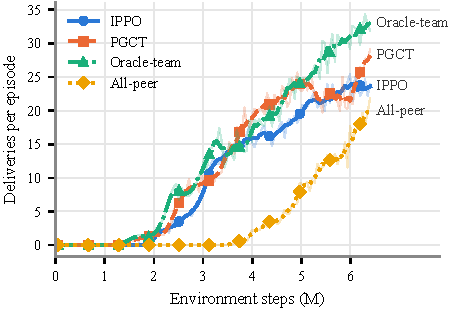
\includegraphics[width=\columnwidth]{figures/fig1_learning_curves.pdf}
\caption{Evaluation deliveries per episode on E1 (one seed\pilot). Thin lines: raw evaluations every 51{,}200 steps;
thick lines: centred 5-point moving average.}
\label{fig:curves}
\end{figure}

\textbf{Learning.} Even when there is no team to discover, \ours{} improved on independent learning on every measure
(Table~\ref{tab:control}, Figure~\ref{fig:curves}):\pilot{} it reached one delivery per episode 0.26M steps (13\%) earlier,
its average throughput over training was 12\% higher (11.7 vs.\ 10.4 deliveries per episode) and its final throughput
18\% higher (27.3 vs.\ 23.2). It was the first method to reach 20 deliveries per episode (4.15M steps vs.\ 4.66M for
Oracle-team and 5.07M for IPPO) and attained 89\% of Oracle-team's average throughput. Indiscriminate sharing delayed
learning: All-peer reached one delivery per episode only after 3.99M steps, although it was improving fastest when the
run ended.

\begin{figure*}[t]
\centering
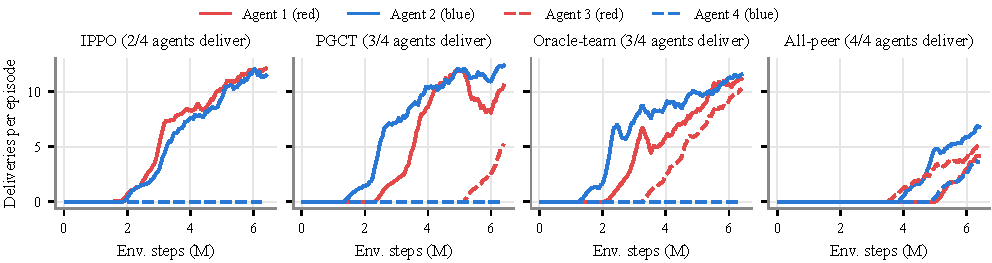
\includegraphics[width=\textwidth]{figures/fig2_per_agent_deliveries.pdf}
\caption{Deliveries per episode of each agent on E1 (5-point moving average; one seed\pilot). Red: team red (agents 1,
3); blue: team blue (agents 2, 4); solid: agents 1--2; dashed: agents 3--4.}
\label{fig:agents}
\end{figure*}

\textbf{Lagging agents.} The per-agent curves (Figure~\ref{fig:agents}) show where the gain comes from. Under IPPO only
one agent per team learned to deliver; the other two kept moving but never picked up a requested shelf. With individual
rewards and two requests per team, the first teammate to learn serves most requests and the second receives too little
reward to learn from. Critic distillation gives the lagging agent a value signal without its own rewards: under \ours{}
and Oracle-team a third agent learned (agent 3, from 5.4M and 3.6M steps), and under All-peer all four did, albeit late.
Each agent that learned contributed about 10--12 deliveries per episode, so the number of learning agents explains most of
the throughput differences. \todo{intervention: block distillation to the lagging agent; count learners over seeds}

\begin{figure*}[t]
\centering
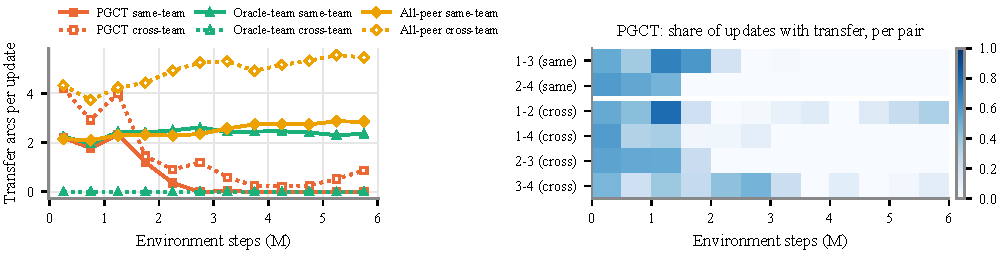
\includegraphics[width=\textwidth]{figures/fig3_critic_transfer.pdf}
\caption{Realised critic transfer on E1 (logged allocation, after warm-up; one seed\pilot). Left: directed transfer arcs
per update within (solid) and across (dotted) teams, in 0.5M-step bins. Right: for \ours{}, share of updates in which each
agent pair exchanged critic information.}
\label{fig:transfer}
\end{figure*}

\textbf{What \ours{} discovers when teams differ only by label.} As expected for this control, the probe distance carried
no team information: from 2.5M steps on, teammates' policies were \emph{less} similar than non-teammates' at almost every
checkpoint and for every method (Figure~\ref{fig:jsgap}), and the same held on frozen models for five probe subsets,
including team-discriminative ones (Appendix~C). Without a team signal, the estimate $\hat{\mathcal{T}}_i$ followed role
and competence instead: after 2M steps it linked agents across teams (agents 3--4, later 1--2; 0.03 same-team vs.\ 0.63
cross-team arcs per update after 4M steps; Figure~\ref{fig:transfer}), namely agents with the same role (staying in the own
half vs.\ fetching shelves from the other half; Appendix~D). This fallback did not hurt in E1: in an independent frozen
evaluation, blending a receiver's critic with a teammate's reduced its value error \emph{less} than blending with a
non-teammate's (same-team AUROC 0.25--0.33), since both teams face the same task. \ours{} also transferred much less than
the baselines after 2M steps (37\% and 29\% of updates vs.\ 82--86\% for Oracle-team and almost 100\% for All-peer). The
control thus establishes two points: \ours{} is not harmed when teams are indistinguishable, and recovering teams
requires an environment in which they behave differently.

\begin{figure}[t]
\centering
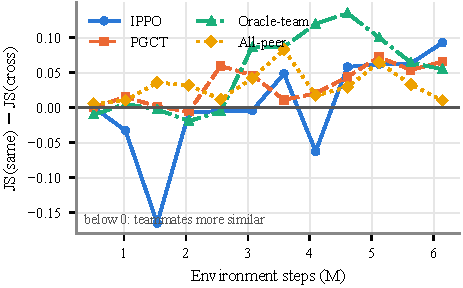
\includegraphics[width=\columnwidth]{figures/fig4_probe_js_gap.pdf}
\caption{Probe distance between teammates minus probe distance between non-teammates on E1 checkpoints (one seed\pilot).
Above zero: teammates' policies differ more than non-teammates'. In the team-symmetric control there is no team signal.}
\label{fig:jsgap}
\end{figure}

\section{Goal-Separated Teams (E1-F)}
\label{sec:main}
\todo{Main results. Fill after the E1-F runs (IPPO, All-peer, Oracle-team, \ours{}, \ours{}-v2; 10M steps; seeds 1--$n$).}
We evaluate the four links of the team-discovery argument in order:
(1) \emph{Does team-restricted sharing pay off?} Oracle-team vs.\ All-peer;
(2) \emph{Are teammates' critics more compatible?} same-team vs.\ cross-team value compatibility on checkpoints;
(3) \emph{Does \ours{} recover the teams?} probe-distance AUROC, share of same-team transfer, and behavioural divergence;
(4) \emph{Does discovery improve learning?} \ours{} and \ours{}-v2 vs.\ IPPO, All-peer and Oracle-team.

\begin{table}[t]
\centering
\small
\resizebox{\columnwidth}{!}{%
\begin{tabular}{lccccc}
\toprule
Method & Onset & Mean & Final & Same-team transfer & Probe AUROC \\
\midrule
IPPO & \tbd & \tbd & \tbd & -- & \tbd \\
All-peer & \tbd & \tbd & \tbd & \tbd & \tbd \\
\ours{} & \tbd & \tbd & \tbd & \tbd & \tbd \\
\ours{}-v2 & \tbd & \tbd & \tbd & \tbd & \tbd \\
Oracle-team & \tbd & \tbd & \tbd & 100\% & \tbd \\
\bottomrule
\end{tabular}}
\caption{Goal-separated task E1-F. Same-team transfer: share of realised transfer arcs between teammates. Probe AUROC:
same-team AUROC of the probe distance on checkpoints. \todo{fill when the runs finish}}
\label{tab:main}
\end{table}

\begin{table}[t]
\centering
\small
\resizebox{\columnwidth}{!}{%
\begin{tabular}{lcccc}
\toprule
 & \multicolumn{2}{c}{E1 ($11\times10$)} & \multicolumn{2}{c}{E2 ($16\times16$)} \\
\cmidrule(lr){2-3}\cmidrule(lr){4-5}
Method & AUC & Last 10 & AUC & Last 10 \\
\midrule
IPPO & 44.57 & 44.52 & 34.24 & 37.61 \\
\ours{} & 45.86 & 46.17 & 34.17 & 37.47 \\
\bottomrule
\end{tabular}}
\caption{Supplementary: continuation for 4M steps from a shared curriculum checkpoint in team-symmetric maps (one
seed\pilot; learning rate $10^{-4}$, entropy coefficient 0.02). When every agent can already deliver, there are no lagging
agents to help and the benefit of \ours{} is small.}
\label{tab:continuation}
\end{table}

\section{Discussion and Limitations}
\textbf{When does team discovery matter?} Team discovery can only help if teams behave differently and if teammates'
value estimates are more useful to each other than non-teammates'. The team-symmetric control satisfies neither, and
there \ours{} behaved like a compatibility-based sharing scheme that still helped lagging agents. Whether both
conditions hold in the goal-separated task, and whether \ours{} then recovers the teams, is the main empirical question
\todo{E1-F}.

\textbf{Preliminary evidence.} All E1 numbers come from one training seed. Re-running the same seed with identical weights
reproduced IPPO exactly but not the sharing variants, which diverged after 1.4--1.6M steps (Appendix~B); in that re-run
All-peer's onset differed by two million steps. Several seeds are therefore required and are running.
\todo{report mean and 95\% interval; identify the non-deterministic operation}

\textbf{Assumptions.} \ours{} assumes a shared probe bank, local communication of model outputs, and observations in which
the same probe means the same situation to all agents. Agents could in principle exchange team identifiers directly; team
discovery is relevant when objectives are private, labels are not shared across organisations, or groups form without a
common vocabulary. Our probe bank is generated by a fixed rule from the map layout; environment-agnostic probe
construction is future work.

\textbf{Scope.} One environment family with four agents and two teams. Larger numbers of agents and teams, team-shared
rewards and centralised baselines (MAPPO, SePS-style and HetDPS-style sharing) are planned. \todo{baselines}

\section{Conclusion}
We introduced \ours{}, a decentralised method in which agents discover latent teammates from their policies' responses to
a shared probe bank and share critics within the discovered team. On a team-symmetric control, where teams cannot be told
apart by behaviour, \ours{} fell back to linking agents with similar roles and still outperformed independent learning and
indiscriminate sharing in a preliminary run, chiefly by letting lagging agents learn. The goal-separated task will show
whether \ours{} recovers teams whose objectives differ and whether team-restricted sharing then improves learning.

\ifdefined\ijcaistyle
  \bibliographystyle{named}
\else
  \bibliographystyle{plainnat}
\fi
\bibliography{references}

\clearpage
\appendix
\onecolumn

\section{Hyper-parameters}
\begin{table}[h]
\centering
\small
\begin{tabular}{ll}
\toprule
Setting & Value \\
\midrule
Map / agents / teams & 11$\times$10 E1 / 4 / 2 \\
Reward & individual \\
Home-zone shelf ratio & 0.5 \\
Requests per team & 2 \\
Sensor / communication range & 5 / 5 \\
Learning rate & 0.0002 \\
Entropy coef. & 0.05 \\
$\gamma$ / GAE $\lambda$ & 0.99 / 0.95 \\
Rollout / BPTT length & 1024 / 64 \\
PPO epochs / minibatches / clip & 4 / 8 / 0.2 \\
Hidden (MLP / GRU) & 128 / 128 \\
Peer-loss coef. $\lambda_{peer}$ & 0.01 \\
Gate: JS threshold / EMA $\beta$ / warm-up & 0.12 / 0.35 / 100 upd. \\
Canonical probes & 48 (fixed, zero hidden, length 1) \\
Evaluation & every 50 updates, 20$\times$500 steps, deterministic \\
\bottomrule
\end{tabular}

\caption{Settings of the from-scratch E1 comparison (identical for all methods except the donor set).}
\end{table}

\section{Reproducibility with an identical seed}
\begin{figure}[h]
\centering
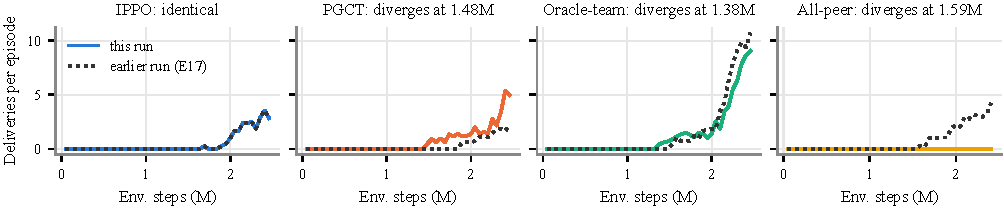
\includegraphics[width=\textwidth]{figures/figA1_reproducibility.pdf}
\caption{Two runs with the same seed and initial weights (solid: reported run; dotted: earlier interrupted run). IPPO is
reproduced exactly; the sharing variants diverge after 1.4--1.6M steps.}
\end{figure}

\section{Probe banks on frozen E1 models}
\begin{figure}[h]
\centering
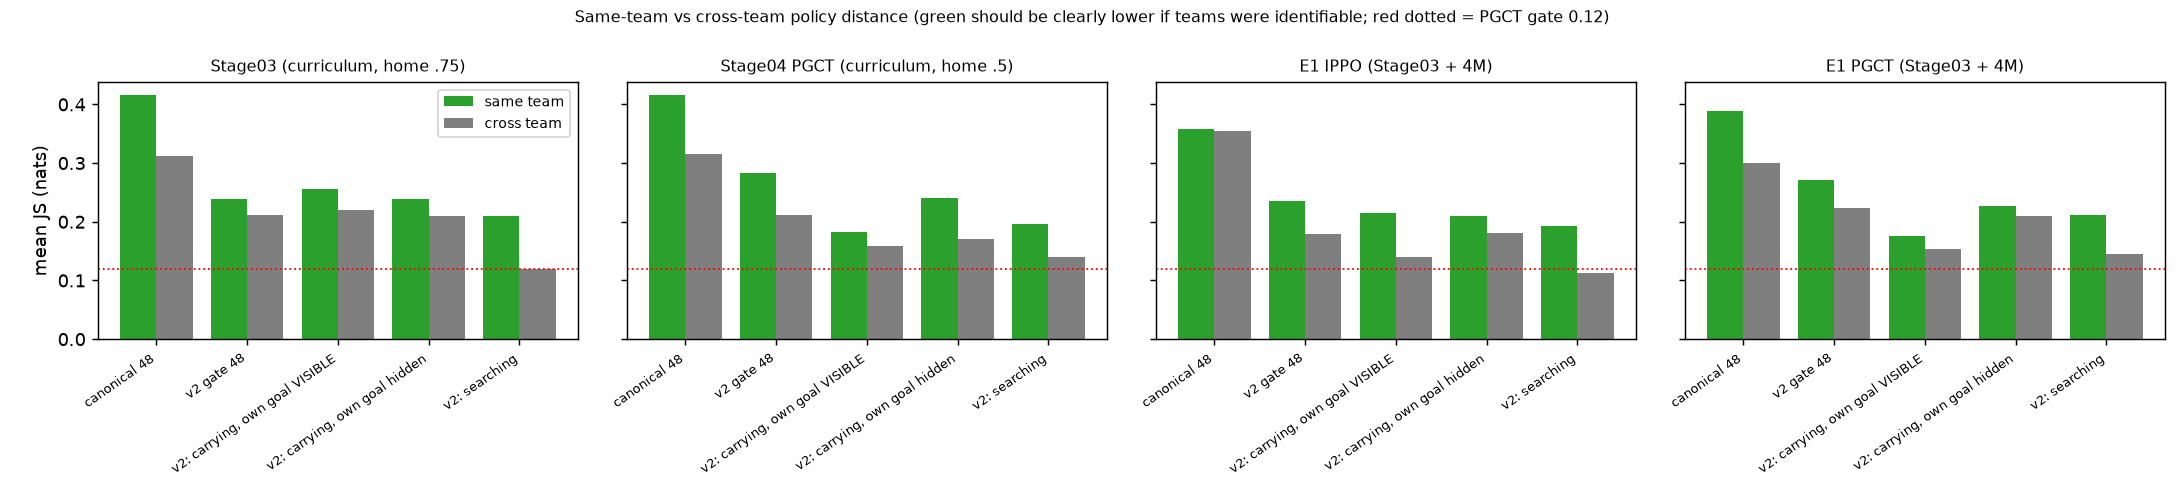
\includegraphics[width=\textwidth]{figures/frozen_probe_same_vs_cross.png}
\caption{Mean probe distance between teammates (green) and non-teammates (grey) for four frozen E1 models and five probe
subsets, including the team-discriminative bank (carrying, no goal in view). In the team-symmetric control teammates are
less similar in all 20 combinations. Red dotted line: threshold 0.12.}
\end{figure}

\section{Roles in a curriculum model}
\begin{figure}[h]
\centering
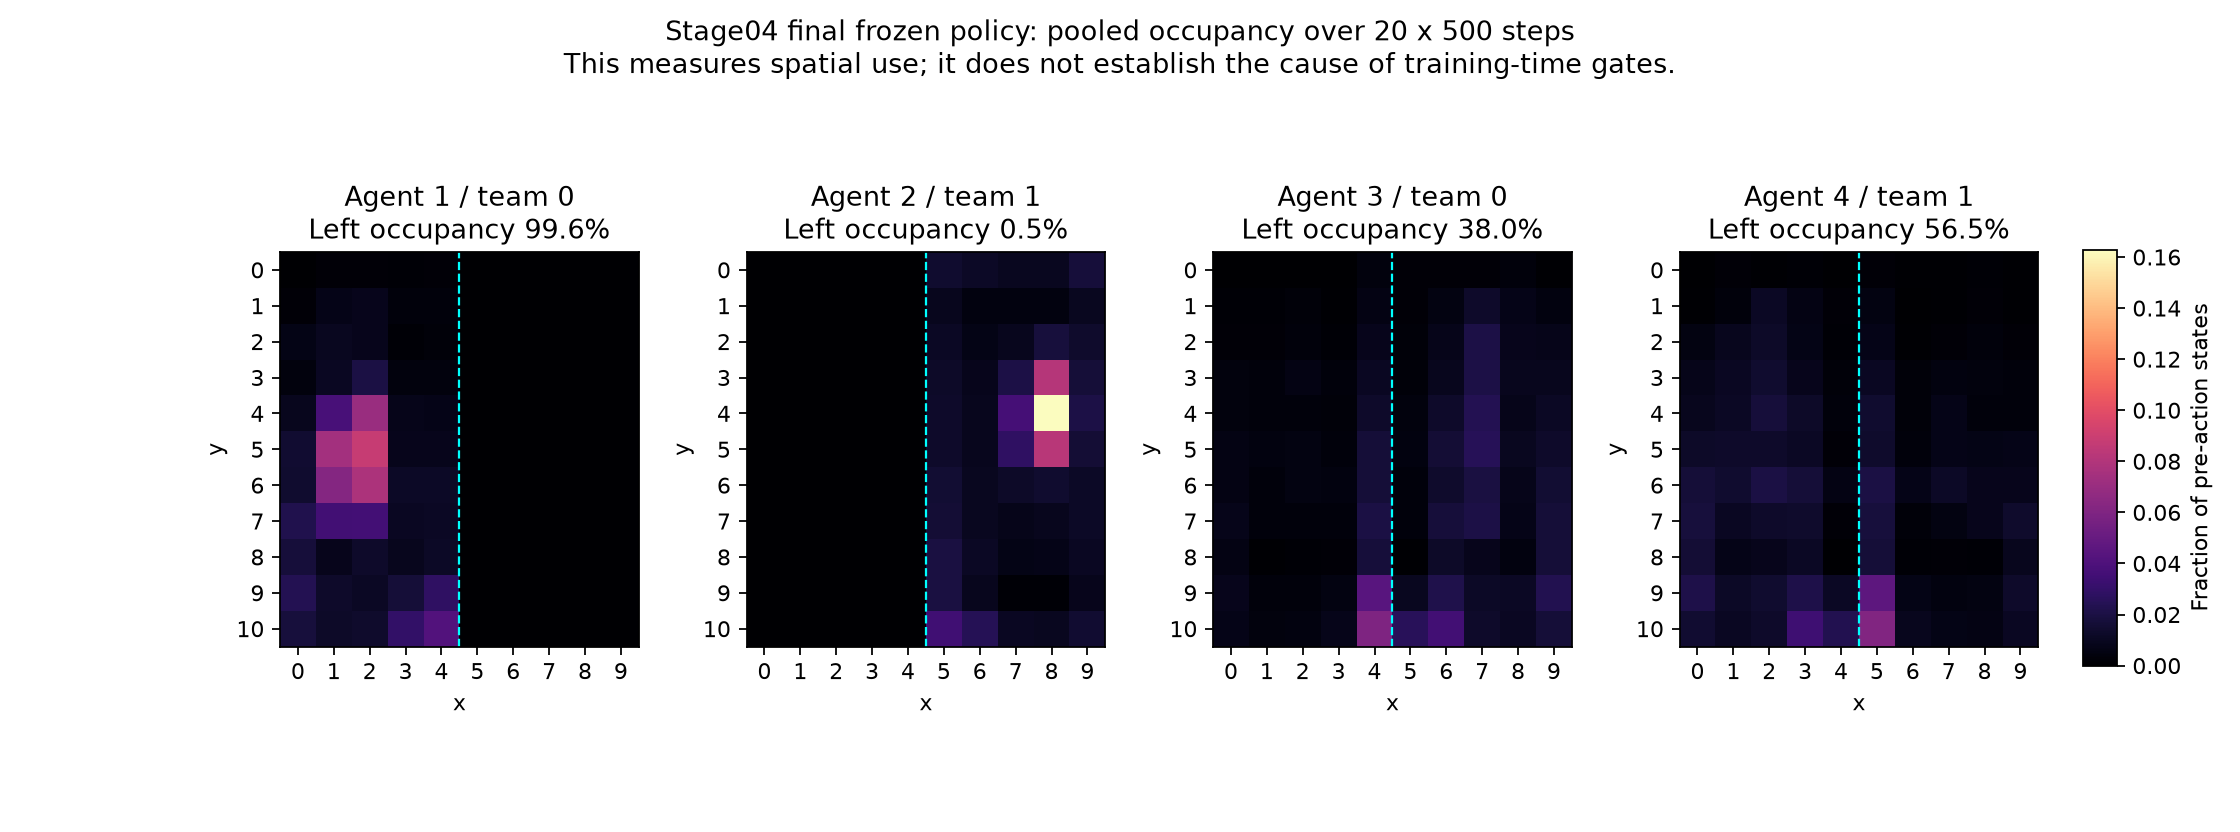
\includegraphics[width=\textwidth]{figures/stage04_occupancy.png}
\caption{Cell occupancy of a frozen curriculum model with 50\% of shelves in the other team's half (20$\times$500 steps).
Agents 1 and 2 stay in their team's half; agents 3 and 4 fetch shelves from the other half and are the pair the gate
linked most often.}
\end{figure}

\section{Realised transfer per window}
\begin{table}[h]
\centering
\small
\begin{tabular}{llccc}
\toprule
Method & Window & Updates w/ transfer & Same-team arcs/upd. & Cross-team arcs/upd. \\
\midrule
PGCT & 0--2.0M & 91\% & 1.86 & 3.09 \\
 & 2--4.0M & 37\% & 0.10 & 0.73 \\
 & 4--6.4M & 29\% & 0.03 & 0.63 \\
\addlinespace
Oracle-team & 0--2.0M & 82\% & 2.26 & 0.00 \\
 & 2--4.0M & 86\% & 2.50 & 0.00 \\
 & 4--6.4M & 85\% & 2.39 & 0.00 \\
\addlinespace
All-peer & 0--2.0M & 99\% & 2.22 & 4.18 \\
 & 2--4.0M & 100\% & 2.49 & 5.10 \\
 & 4--6.4M & 100\% & 2.79 & 5.37 \\
\bottomrule
\end{tabular}

\caption{Realised transfer on E1 per training window (one seed). Arcs are directed receiver--donor links.}
\end{table}

\end{document}
